\section{Projektmonitoring}
\label{sec:Projektmonitoring}

\subsection{Auswertung Velocity}
\label{sub:Auswertung Velocity}

\begin{figure}[H]
    \centering
    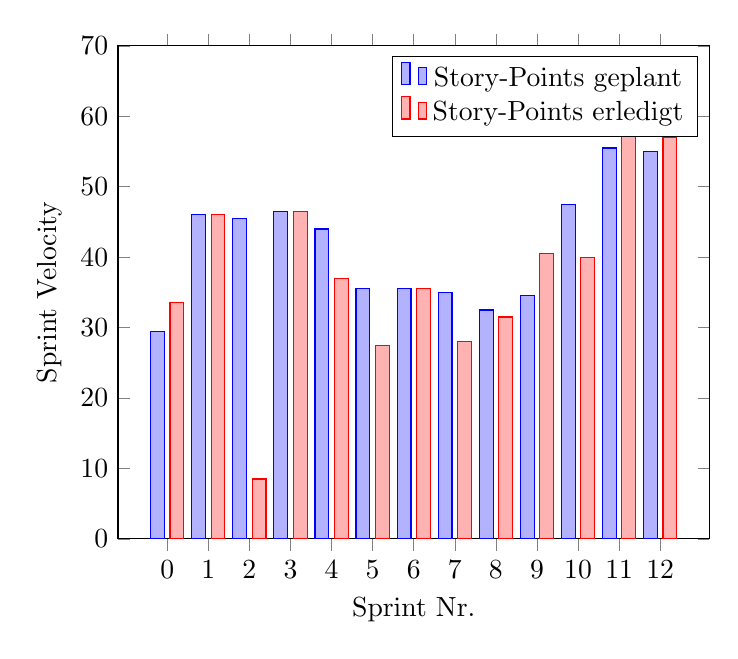
\begin{tikzpicture}
        \begin{axis}[
            ybar,
            width=0.75\textwidth,
            bar width=5pt,
            ylabel={Sprint Velocity},
            xlabel={Sprint Nr.},
            ymin=0,
            ymax=70,
            xtick=data,
            % nodes near coords,
            % nodes near coords align={vertical},
            % every node near coord/.append style={color=black, font=\tiny}
        ]
            \addplot[style={blue, fill=blue!30!white}] coordinates
                {(0, 29.5) (1, 46) (2, 45.5) (3, 46.5) (4, 44) (5, 35.5) (6, 35.5) (7, 35)
                (8, 32.5) (9, 34.5) (10, 47.5) (11, 55.5) (12, 55)};
            \addplot [style={red, fill=red!30!white}] coordinates
                {(0, 33.5) (1, 46) (2, 8.5) (3, 46.5) (4, 37) (5, 27.5) (6, 35.5) (7, 28)
                (8, 31.5) (9, 40.5) (10, 40) (11, 60.5) (12, 57)};
            \legend{Story-Points geplant,Story-Points erledigt}
        \end{axis}
    \end{tikzpicture}%

    \caption[Diagramm Velocity über das Projekt]{Sprint Velocity über den Verlauf des Projekts}
    \label{chart:sprint_velocity}
\end{figure}


\subsection{Zeitauswertung}
\label{sub:Zeitauswertung}

\begin{figure}[H]
    \centering
    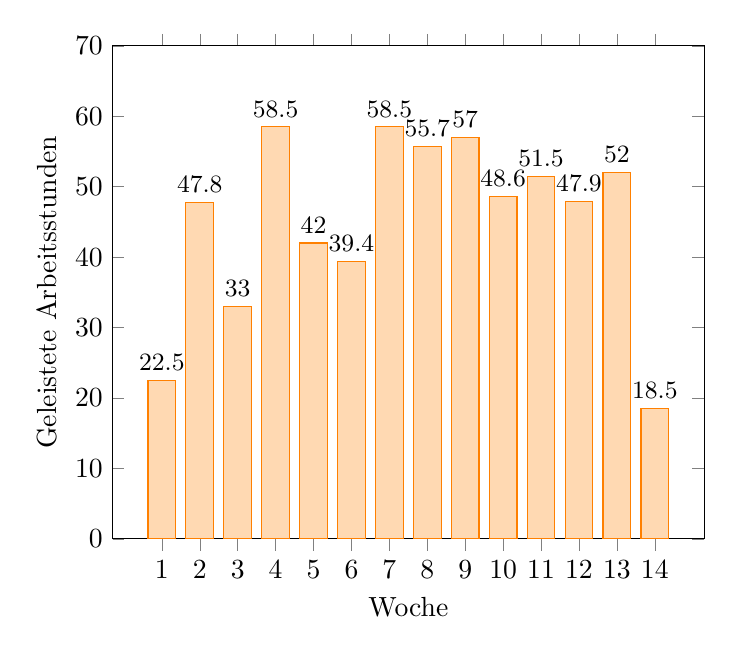
\begin{tikzpicture}
        \begin{axis}[
            ybar,
            width=0.75\textwidth,
            bar width=10pt,
            ylabel={Geleistete Arbeitsstunden},
            xlabel={Woche},
            ymin=0,
            ymax=70,
            xtick=data,
            nodes near coords,
            nodes near coords align={vertical},
            every node near coord/.append style={color=black, font=\small}
        ]
            \addplot[style={orange, fill=orange!30!white}] coordinates
                {(1, 22.5) (2, 47.8) (3, 33) (4, 58.5) (5, 42) (6, 39.4) (7, 58.5)
                (8, 55.7) (9, 57) (10, 48.6) (11, 51.5) (12, 47.9) (13, 52) (14, 18.5)};
        \end{axis}
    \end{tikzpicture}

    \caption[Diagramm Zeitaufwand über den Verlauf des Projekts]{Zeitaufwand über den Verlauf des Projekts (Stand 19.12.2017)}
    \label{chart:Zeitauswertung}
\end{figure}


\subsection{Codestatistik}
\label{sub:Codestatistik}
